\documentclass[tikz,border=8pt]{standalone}
\usepackage[T1]{fontenc}
\usepackage{times}
\usepackage{amsmath,amssymb}
\usetikzlibrary{positioning,arrows.meta,fit,backgrounds,calc,shapes.geometric}
\definecolor{encC}{HTML}{4C72B0}
\definecolor{decC}{HTML}{DD8452}
\definecolor{subsC}{HTML}{5A9E6F}
\definecolor{darkC}{HTML}{343434}
\definecolor{faintC}{HTML}{F2F2F2}
\begin{document}
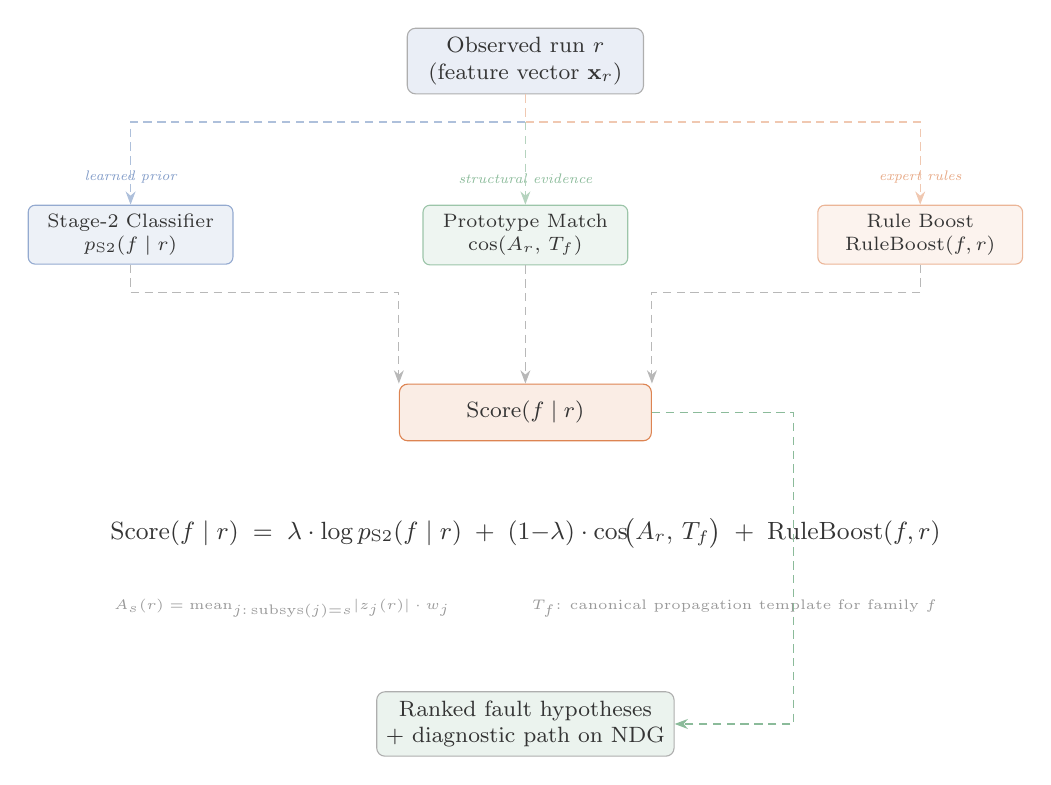
\begin{tikzpicture}[
  >=Stealth,
  every node/.style={font=\rmfamily\small, text=darkC},
  block/.style={draw=darkC!40, fill=#1!12, rounded corners=3pt,
                minimum width=3.0cm, minimum height=0.72cm,
                font=\rmfamily\footnotesize, align=center},
  opbox/.style={draw=#1!60, fill=#1!10, rounded corners=2.5pt,
                minimum width=2.6cm, minimum height=0.6cm,
                font=\rmfamily\scriptsize, align=center},
  scorebox/.style={draw=decC, fill=decC!15, rounded corners=3pt,
                   minimum width=3.2cm, minimum height=0.72cm,
                   font=\rmfamily\footnotesize, align=center},
]

% ── Input ──
\node[block=encC] (run) {Observed run $r$\\(feature vector $\mathbf{x}_r$)};

% ── Three parallel channels ──
\node[opbox=encC, below left=1.4 and 2.2 of run] (s2)
  {Stage-2 Classifier\\$p_{\text{S2}}(f \mid r)$};
\node[opbox=subsC, below=1.4 of run] (sig)
  {Prototype Match\\$\cos(A_r,\, T_f)$};
\node[opbox=decC, below right=1.4 and 2.2 of run] (rule)
  {Rule Boost\\$\text{RuleBoost}(f,r)$};

% ── Channel labels ──
\node[font=\rmfamily\tiny\itshape, text=encC!70,
      above=0.15 of s2] {learned prior};
\node[font=\rmfamily\tiny\itshape, text=subsC!70,
      above=0.15 of sig] {structural evidence};
\node[font=\rmfamily\tiny\itshape, text=decC!70,
      above=0.15 of rule] {expert rules};

% ── Arrows from run to channels (light dashed to avoid obscuring labels) ──
\draw[->, densely dashed, encC!45] (run.south) -- ++(0,-0.35) -| (s2.north);
\draw[->, densely dashed, subsC!45] (run.south) -- (sig.north);
\draw[->, densely dashed, decC!45] (run.south) -- ++(0,-0.35) -| (rule.north);

% ── Score box ──
\node[scorebox, below=1.5 of sig] (score) {$\text{Score}(f \mid r)$};

% ── Arrows from channels to Score (light dashed to not cut through text) ──
\draw[->, densely dashed, darkC!35] (s2.south) -- ++(0,-0.35) -| (score.north west);
\draw[->, densely dashed, darkC!35] (sig.south) -- (score.north);
\draw[->, densely dashed, darkC!35] (rule.south) -- ++(0,-0.35) -| (score.north east);

% ── Equation (definition block) ──
\node[font=\small, text=darkC, below=0.85 of score] (eq) {%
  $\displaystyle \text{Score}(f \mid r) \;=\;
   \lambda \cdot \log p_{\text{S2}}(f \mid r)
   \;+\; (1{-}\lambda)\cdot\cos\!\bigl(A_r,\, T_f\bigr)
   \;+\; \text{RuleBoost}(f,r)$};

% ── Definitions ──
\node[font=\rmfamily\tiny, text=darkC!50, below=0.4 of eq, align=center] (defs) {%
  $A_s(r) = \displaystyle\operatorname{mean}_{j:\,\text{subsys}(j)=s}
   \lvert z_j(r)\rvert \cdot w_j$
  \qquad\qquad
  $T_f$: canonical propagation template for family $f$};

% ── Output ──
\node[block=subsC, below=0.8 of defs] (out)
  {Ranked fault hypotheses\\+ diagnostic path on NDG};

% ── Arrow from Score to Output, routed far right to avoid equation ──
\draw[->, densely dashed, subsC!70]
  (score.east) -- ++(1.8,0) |- (out.east);

\end{tikzpicture}
\end{document}
